% Course report, using the unchanged official AAAI 2026 style in draft mode.
% Metrics and comparison rows are generated only from completed local runs.
\documentclass[letterpaper]{article}
\usepackage[draft]{aaai2026}
\usepackage{times}
\usepackage{helvet}
\usepackage{courier}
\usepackage[hyphens]{url}
\usepackage{graphicx}
\usepackage{natbib}
\usepackage{caption}
\usepackage{amsmath}
\usepackage{iftex}
\ifXeTeX
  \usepackage[OT1]{fontenc}
  \let\pdfpagewidth\paperwidth
  \let\pdfpageheight\paperheight
  \providecommand{\pdfinfo}[1]{\special{pdf:docinfo <<#1>>}}
\fi
\urlstyle{rm}
\def\UrlFont{\rm}
\frenchspacing
\setlength{\pdfpagewidth}{8.5in}
\setlength{\pdfpageheight}{11in}
\pdfinfo{/TemplateVersion (2026.1)}
\setcounter{secnumdepth}{0}
\title{Parameter-Efficient Residual Classification with PyramidNet and Weight Averaging}
\author{Sheng Tao}
\affiliations{NYU Tandon School of Engineering\\Deep Learning, Fall 2026\\
\url{https://github.com/TolsonRyan/cifar10-resnet-architecture-challenge}}
\begin{document}
\maketitle
\begin{abstract}
We investigate CIFAR-10 image classification with a residual convolutional network constrained to fewer than five million trainable parameters. Our final model is a locally implemented PyramidNet-110 with ShakeDrop regularization and 4,804,512 parameters. A shared model is trained from random initialization for 400 epochs, followed by two 20-epoch continuations with different random seeds. We average the final branch weights into one inference network and average its class probabilities across 50 translated and horizontally flipped views. The resulting model achieves 97.90\% on a repeatedly used 5,000-image development split and 87.60\% on the competition's final hidden evaluation subset. Controlled comparisons show modest development improvements from continuation and test-time augmentation, while also exposing the limits of interpreting small improvements after repeated model selection.
\end{abstract}

\section{Overview}
The project requires a modified ResNet trained from scratch using only the permitted CIFAR-10 training images, with at most 5,000,000 trainable parameters. Residual connections allow the model to learn transformations around an identity path rather than repeatedly reconstructing its input representation \citep{he2016resnet}. Under a parameter budget, increasing width competes with depth and training cost. Our final design uses gradual channel growth rather than abrupt channel doubling at every stage boundary.

The contribution of this course project is an implemented and measured training and inference pipeline, not a claim of a new architecture. We combine a parameter-constrained PyramidNet, stochastic residual regularization, deterministic short continuation, fixed weight averaging, and test-time augmentation. All reported local measurements come from completed runs. No external training images, pretrained weights, or hidden test labels were used.

\section{Methodology}
\subsection{Data and evaluation protocol}
The provided data contain 50,000 labeled 32$\times$32 RGB training images and 2,000 unlabeled competition images. We use a stratified split generated with seed 2026: 45,000 training examples and 5,000 validation examples, respectively 4,500 and 500 per class. The final model and both continuation branches use this same training subset. Validation examples are excluded from gradient updates and normalization statistics.

Images are loaded as RGB uint8 arrays, converted to floating point in $[0,1]$, and normalized using training-only channel means $(0.491514,0.482315,0.446814)$ and standard deviations $(0.247051,0.243480,0.261510)$. Predictions follow the official sample submission ID order. Checks enforce image shape, channel format, unique IDs, and integer labels from zero through nine.

The validation split was used repeatedly to select configurations and inference policies. It is therefore a development set, not an untouched test set. The final test accuracy is the official hidden final-evaluation result reported by the participant; its labels are unavailable locally. We do not infer test accuracy from prediction confidence or from synthetic perturbations.

\subsection{Residual architecture}
PyramidNet gradually increases channel width across residual blocks \citep{han2017pyramid}. Our network has a 16-channel $3\times3$ stem and 54 basic residual blocks, with 18 blocks in each spatial stage. The output width of block $i$ is
\[
 c_i=\operatorname{round}(16+96i/54),\qquad i=1,\ldots,54.
\]
The resulting stage-end widths are 48, 80, and 112. Each block applies input batch normalization (BN), a $3\times3$ convolution, BN and ReLU, another $3\times3$ convolution, output BN, and ShakeDrop before adding the shortcut. There is no post-addition ReLU. The first block in stages two and three downsamples by two. Its shortcut uses average pooling; additional channels are zero-padded. Thus every block retains an explicit residual addition without a learned projection on the shortcut. Final BN, ReLU, global average pooling, and a ten-class linear layer complete the model.

\begin{table}[t]
\centering
\begin{tabular}{lrr}
\hline
Component & Channels & Resolution\\\hline
Stem &16&$32\times32$\\
Stage 1: 18 blocks&48&$32\times32$\\
Stage 2: 18 blocks&80&$16\times16$\\
Stage 3: 18 blocks&112&$8\times8$\\
Pooling + classifier&10&--\\\hline
\end{tabular}
\caption{Final residual architecture. Parameter count, including BN affine parameters and the classifier, is 4,804,512.}
\end{table}

Gradual growth distributes capacity across depth while zero-padding shortcuts avoid extra projection parameters. Compared with a wider, shallower residual network, this design requires more sequential operations and longer training. We selected the complete recipe empirically; the experiments do not isolate architectural effects from training duration and regularization.

\subsection{Base training}
The shared base is trained for 400 epochs using SGD with Nesterov momentum 0.9, batch size 128, weight decay $10^{-4}$, and initial learning rate 0.1. Five warmup epochs precede per-step cosine decay to approximately $10^{-4}$. Training uses BF16 on an RTX 4060 Laptop GPU with 8 GB memory; evaluation uses FP32 with TF32 disabled.

Augmentation consists of reflection-padding by four pixels, random $32\times32$ crops, horizontal flips, RandAugment with two operations and magnitude nine, and Cutout with side length 16 \citep{cubuk2020randaugment,devries2017cutout}. RandAugment operation choices are shared within shuffled groups of 32 images; crop, flip, and Cutout locations are sampled per image. Cutout is applied after normalization and fills the masked region with zero. This implementation detail is preserved in the reproduction code. Mixup, CutMix, and label smoothing are not active in the final recipe.

ShakeDrop perturbs the residual branch during base training \citep{yamada2019shake}. Block death probabilities increase linearly to 0.5. A batch-level Bernoulli gate and per-image forward and backward coefficients provide the stochastic residual multipliers. At inference the residual is multiplied by its keep probability. An exponential moving average (EMA) with target decay 0.999 tracks floating model tensors, including BN statistics; integer buffers are copied. Its initial decay is bounded by $(1+u)/(10+u)$ at update $u$.

\subsection{Two continuation branches and averaging}
Both branches start from the base model's epoch-400 EMA weights. Seeds 62026 and 62029 determine their subsequent randomness. Each runs for 20 epochs with fresh SGD momentum, learning rate 0.002 decaying to approximately 0.0001, and the same data augmentation and weight decay. During continuation, only ShakeDrop modules use their deterministic inference multiplier; BN remains in training mode. This reduces residual-branch stochasticity without changing the deployed network.

We use the final Raw endpoints, not the highest-scoring intermediate epoch. All floating tensors are averaged with fixed equal weights,
\[
 \bar\theta=(\theta_A+\theta_B)/2.
\]
This includes BN running means and variances. Integer buffers are retained from branch B, and no subsequent BN recalibration is applied. This is a two-branch weight average, related to weight-averaging approaches \citep{izmailov2018averaging}, rather than a prediction ensemble or an implementation of standard stochastic weight averaging. Only one network is deployed. Each branch follows a 420-epoch path; the shared computation is 400 base epochs plus two separate 20-epoch continuations.

\subsection{Test-time augmentation}
We reflection-pad the input by two pixels and use every integer translation in $\{-2,-1,0,1,2\}^2$, with and without a horizontal flip. The 25 translations produce 50 views. Normalization is applied after forming each view. We average probabilities rather than logits:
\[
 p(y\mid x)=\frac1{50}\sum_{v=1}^{50}
 \operatorname{softmax}(f_{\bar\theta}(T_v(x))).
\]
The view weights are uniform and are not fitted to hidden test data. The policy preserves a fixed ordering and uses FP32 inference with batch size 64. It increases forward-pass cost while leaving the parameter count unchanged.

\section{Results}
\subsection{Controlled final-model comparisons}
Table~\ref{tab:results} compares checkpoints and inference policies on the same validation examples. Raw denotes the live trained weights, while EMA denotes their moving average. All continuation endpoints are fixed at epoch 20.
\begin{table}[t]
\centering\small
\begin{tabular}{lrrr}
\hline
Weights & Views & Accuracy (\%) & NLL\\\hline
Base EMA400 &1&97.48&0.08292\\
Base EMA400 &10&97.70&0.07459\\
Branch A Raw &10&97.86&0.07267\\
Branch B Raw &10&97.82&0.07307\\
Two-branch average &10&97.86&0.07264\\
Two-branch average &18&97.90&0.07194\\
Two-branch average &50&97.90&0.07172\\\hline
\end{tabular}
\caption{Measured development results. All models use the same 45,000 training images and 4,804,512 parameters. The 18-view policy uses offsets $\{-2,0,2\}^2$ and flips.}
\label{tab:results}
\end{table}

The base EMA model gains 0.22 percentage points from ten-view inference. Continuation branch A adds a further 0.16 points under the same policy, while branch B reaches a similar result. Equal weight averaging preserves branch A's accuracy but does not improve it under ten views. With 50 views, the averaged model correctly classifies 4,895 of 5,000 validation images. Relative to its ten-view prediction, five examples become correct and three become incorrect. The 18-view and 50-view policies have equal accuracy; their disagreements exchange three correct predictions in each direction. These are small changes, not evidence of statistical significance.

\begin{figure}[t]
\centering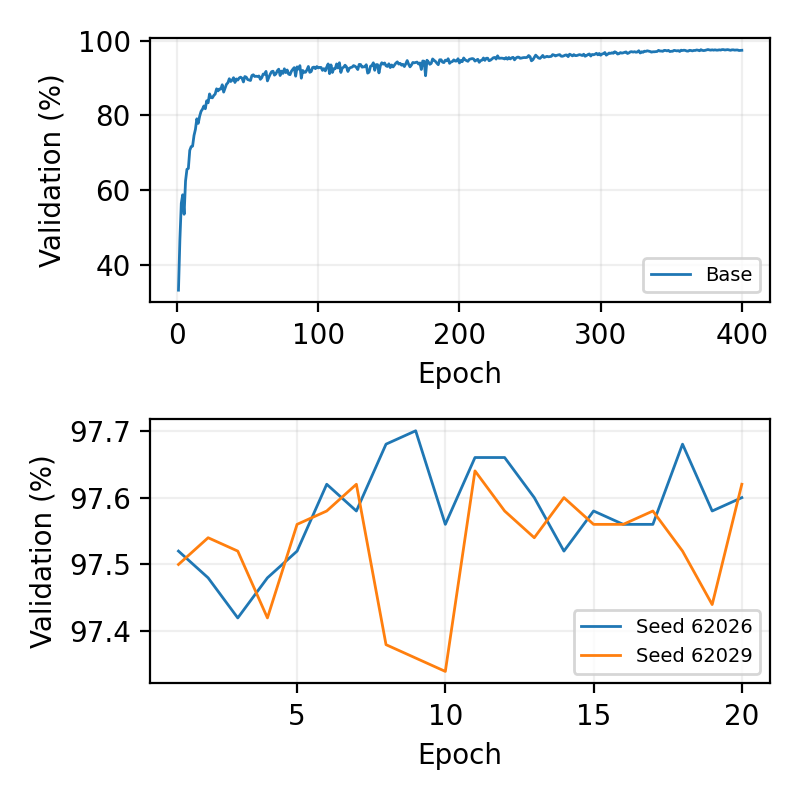
\includegraphics[width=\columnwidth]{final_training.png}
\caption{Recorded validation trajectories for the shared base and two continuation branches. Separate axes avoid presenting the branches as one continuous trajectory.}
\end{figure}

\subsection{Robustness diagnostics and final evaluation}
The existing diagnostic suite applies seven controlled transformations to validation images: brightness scaling by 0.7 and 1.3, contrast scaling by 0.6, grayscale conversion, Gaussian noise with standard deviation 0.05, Gaussian blur with sigma 0.7, and a two-pixel translation. For the averaged model, mean accuracy across these conditions is 94.6371\% with ten views, 94.7057\% with 18 views, and 94.7543\% with 50 views. These conditions are not independent test datasets and do not identify the hidden evaluation distribution.

\begin{table}[t]
\centering
\begin{tabular}{lr}\hline
Final-model measure & Value\\\hline
Trainable parameters &4,804,512\\
Training images &45,000\\
Development accuracy &97.90\%\\
Official final test accuracy &87.60\%\\\hline
\end{tabular}
\caption{Final submitted model. Official test accuracy refers to the competition's final hidden evaluation subset, as confirmed by the participant. It is distinct from local development accuracy.}
\end{table}

The submitted prediction file contains exactly 2,000 rows in official ID order. Its stored checkpoint and CSV hashes allow independent reproduction checks. The original export took approximately 64 seconds for the 2,000 images on the project GPU, excluding image loading and model setup. The shared base and two branches required approximately 7.86 hours of recorded training-workflow time, excluding earlier exploratory experiments. These measurements are hardware- and implementation-specific.

\section{Discussion and Limitations}
The final model satisfies the parameter budget while retaining 54 residual connections. Weight averaging compresses two nearby trained endpoints into a single inference state; it does not double the deployed parameter count. However, the observed benefit is modest, and 50-view inference is substantially more expensive than one-view inference. The results support this particular measured recipe, not a general claim that more views always improve accuracy.

The 10.30-percentage-point difference between development and final test accuracy limits conclusions drawn from local model selection. The development split was repeatedly inspected, the two branches share their base and training examples, and no new untouched validation partition was used for the final selection. We cannot establish the cause of the hidden-test gap without labels or distribution information. We therefore avoid attributing it to a specific corruption or to overfitting alone.

Several design choices were changed together during earlier exploration. This report focuses on the reproducible final-model comparisons rather than presenting those changes as isolated architecture ablations. Synthetic stress averages are supplementary diagnostics, not substitutes for held-out test performance. CUDA execution is not guaranteed bitwise deterministic during retraining; exact submitted-file reproduction instead uses the archived final checkpoint and fixed inference configuration.

\section{Conclusion}
A gradually widened residual network with ShakeDrop, short deterministic-residual continuation, and fixed weight averaging yields a compliant 4.80-million-parameter classifier. The final model reaches 97.90\% development accuracy and 87.60\% official final test accuracy. The most useful finding is the distinction between small, measurable development improvements and uncertain generalization gains. The accompanying code, executed notebook, configurations, and checkpoint provenance make that distinction inspectable and the submitted predictions reproducible.

\section*{Implementation and Tool Disclosure}
The implementation uses PyTorch. RandAugment operations are adapted from torchvision with its BSD-3-Clause notice retained. Codex assisted with implementation, debugging, experiment execution, analysis, and manuscript preparation. Sheng Tao is the sole author and is responsible for reviewing the methods and results. No external pretrained weights or training data were used. Detailed sources and reproduction instructions are included in the repository.
\bibliography{references}
\end{document}
